
\section{Key Performance Indicators (KPIs)}

The following Key Performance Indicators (KPIs) show how OpenDreamKit addresses the specific impacts listed in the work
programme. KPIs were thought through by the members of OpenDreamKit so that they are meaningful, reusable, realistic and easily measurable.
the following qualitative and quantitative indicators are divided into the four aims of OpenDreamKit. If quantitative indicators are more
useful for reporting and internal evaluation, qualitative indicators will give content for father dissemination and communication purposes,
for example through the project website.


\subsection{KPIs for Aim 1}

\begin{aim}
  Improve the productivity of researchers in pure mathematics and
  applications by promoting collaborations based on mathematical
  software, data, and knowledge.
\end{aim}

\subsubsection{Success story}

\begin{enumerate}
\item RP2 \textbf{How OpenDreamKit supported the RSE revolution}\\
  In a \href{https://opendreamkit.org/2018/10/29/ODK-RSE/}{blog post}
  on October 2018, OpenDreamKit fellow Mike Croucher describes How
  OpenDreamKit supported the RSE revolution, saying that "By 2015,
  there were a small number of central ‘Research Software Engineering
  Groups’ within UK Universities with his group at Sheffield being
  among the first. OpenDreamKit was one of the first projects they won
  that demonstrated that funders would support RSEs on major grants –
  this improved credibility of the new role a great deal and helped
  secure its future at Sheffield."

  \noindent
  Mike Croucher is a Research Software Engineer at the university
  of Sheffield, passionate about improving the quality of research
  software. He enables researchers to ask larger and more complex
  research questions by improving the software they develop. Along
  with the Software Sustainability Institute, the UK Research Software
  Engineering Association and the EU-funded OpenDreamKit project,
  Mike Croucher actively campaign to improve the career prospects
  of the talented people who underpin a huge amount of computational
  research….
\end{enumerate}

\subsection{KPIs for Aim 2 and adoption of \ODK's technologies}

\begin{aim}
  Make it easy for teams of researchers of any size to set up custom,
  collaborative Virtual Research Environments tailored to their
  specific needs, resources and workflows. The VRE should support the
  entire life-cycle of computational work in mathematical research,
  from initial exploration to publication teaching and outreach;
\end{aim}

%\paragraph*{Success story: \ODK based VRE deployments} %  and generally speaking adoption of \ODK's components.

\subsubsection{Success stories}
\begin{enumerate}
\item RP2 \textbf{Jupyter's ACM Software System award}\\
  In June 2018,
  \href{https://blog.jupyter.org/jupyter-receives-the-acm-software-system-award-d433b0dfe3a2}{Jupyter
    was awarded prestigious 2017 ACM Software System}. Award previous
  winners include: UNIX, TCP/IP, the Web, TeX, Java, GCC, LLVM.

\item RP2, RP3 \textbf{Partnership with EGI}\\
  there is an ongoing collaboration between EGI (main stakeholder of
  the EOSC) and OpenDreamKit to deploy JupyterHub and BinderHub-based
  EGI services. Proofs of concepts for both have been
  deployed.% by Enol Fernandez from EGI.
  Both parties are very satisfied with the collaboration and want to
  strengthen it. A Technology Provider Agreement was signed between
  EGI and Simula, on behalf of OpenDreamKit/Jupyter developers, and a
  joint application submitted to the EOSC call INFRAEOSC-02-2019.
%https://github.com/OpenDreamKit/OpenDreamKit.github.io/blob/7cbee70c3bff6d0778733be931c927981df87e65/meetings/2018-10-28-Luxembourg/SteeringCommitteeMeeting/ProgressReports/ParisSud.md
%https://github.com/OpenDreamKit/OpenDreamKit/blob/88ee2544e31e661c4eac7f39fa7333f24b62ab2a/WP4/D4.8/report.tex

\item RP2 \textbf{Use of Jupyter components by Logilab's Simulagora}\\
  %
  One of the flagship product of Logilab is Simulagora, an
  industry-grade VRE for collaborative computational simulation; it
  eases the deployment of micro web applications to leverage the
  access to complex simulations to end users. Since Logilab joined
  OpenDreamKit, it was able to outsource several of the core
  components of Simulagora to replace them by analog standard Jupyter
  components, bringing in more interactivity.

\item RP2: \textbf{Blogs about how to deploy Jupyter-based VREs}
  \begin{itemize}
  \item Luca De Feo: \href{https://opendreamkit.org/2018/10/17/jupyterhub-docker/}{Deploying a containerized JupyterHub server with Docker}
  \item Nicolas Thiéry: \href{https://opendreamkit.org/2018/03/15/jupyterhub-binder-convergence/}{Toward versatile JupyterHub deployments, with the Binder and JupyterHub convergence}
  \item Loic gouarin: \href{https://blog.jupyter.org/how-to-deploy-jupyterhub-with-kubernetes-on-openstack-f8f6120d4b1}{Deploying JupyterHub with Kubernetes on OpenStack}
  \end{itemize}

\item RP3: \textbf{Multiple European Binder instances run as a free service for the community}

\label{}
  
Multiple instances of the Binder VRE-deployment tool
are deployed throughout the world,
which can leverage ODK components.
In addition to the original deployment by the Binder team,
sponsored by Google Cloud,
French cloud provider OVH
and GESIS,
the Liebniz institute for Social Sciences in Germany,
sponsor and operate instances in the Binder Federation.
Additionally,
The UK-based Turing Institute is joining the Binder Federation by the end of 2019.
This is an indication of the wide adoption of the Jupyter ecosystem for VRE-deployment,
and an indicator of the strong choice made by ODK
to center much of the work on Jupyter; thanks to this choice,
users of ODK components immediately benefit
from developments such as the Binder service.


%As part of the Open Dream Kit project, Logilab is working on the creation of tools for mesh data visualization and analysis in a web application. The goal was to create widgets to use in Jupyter notebook (formerly IPython) for 3D visualization and analysis. They want to create a graphical user interface in order to enable users to intuitively compute multiple effects on their meshes.

%Simulagora.com, a virtual research environment has been under heavy development since the summer 2017 and a new version is online since March 2018. This showcases the virtual desktops available from a web browser and collaboration workflows based on “tools” that can be described as micro web applications that require very little development skills to set up, but make it easy to make available complex simulations to users.


%Use of ODK's computational components in collaborative workspaces: A group of mathematical researchers with access to common computational resources, such as a shared lab computer or cloud servers, has already been able to deploy a prototype VRE with JUPYTERHUB, integrating OpenDreamKit components. The Jupyter kernels for mathematical software developed as part of OpenDreamKit make computational mathematical components accessible in a JUPYTER environment, enabling a Jupyter-based deployment of the relevant tools for the researchers. The process of working on notebooks is greatly improved by review tools developed as part of WP4, enabling researchers to collaborate to some degree in a shared computational environment.

\item RP2,3 \textbf{Multi-Site involvement of Researchers (Mobility of Researchers)}\\
  The excellent collaboration between the \ODK partners has led to an
  increased mobility of researchers. Rehires between partners and
  joint appointments are a good measure of this:
  \begin{compactitem}
  \item PD. Dr. Florian Rabe (Joint appointment UPSud/FAU)
  \item Felix Schmoll Summer Internship (From JacU to St.Andrews)
  \item Prof. Nathan Carter (Bentley Univ.) in St. Andrews (Sabbatical)
  \end{compactitem}
\item RP2: \textbf{A MitM- and OpenDreamKit-inspired initiative in the theorem proving community}\\
  Logipedia (\url {http://logipedia.science}) was launched in 2018 and aims at integrating proof assistants in a way similar to what OpenDreamKit did for computation systems.
  The FAU site of OpenDreamKit has collaborated with the group behind Logipedia throughout OpenDreamKit, and several ideas of OpenDreamKit, especially the MitM approach, are closely related to the ideas underlying Logipedia.
  An EU-infrastructure proposal centered around Logipedia (with participation of FAU) is in preparation.
\item RP3: \textbf{Immediate Community Building around \dmh}\\
    At the Math Data Workshop in Cernay in August 2019  we invited two external
    researchers who specialize in mathematical datasets in combinatorics. They contributed
    five datases (data, descriptions, schema theories, and provenance) for inclusion in
    \dmh and have been active after the workshop. They indenpendently recruited two of
    their colleagues for the Slack channel that focuses the nascent community. 
\end{enumerate}

\subsubsection{Quantitative metrics}
\begin{enumerate}
\item \textbf{\ODK based VRE deployments}\\
  We are
  \href{https://github.com/OpenDreamKit/OpenDreamKit/issues/174}{tracking}
  collaborations with various institutions and projects to deploy
  instances of JupyterHub and CoCalc (formerly SageMathCloud). There
  are \textbf{nice major OpenDreamKit based VRE deployments} so far:
  seven at the scale of academic institutions (universities of Zurich,
  Paris Sud / Paris Saclay, Sheffield, UVSQ, Gent, University of Oslo, NTNU), and two at the
  scale of research networks (EGI, Mathrice). See
  Section~\ref{infrastructures} for details.

  There are many more than those listed above; however due to the VRE
  toolkit approach and its success, it is hard to track them: indeed
  \ODK members need not be contacted or involved in any such
  deployments. This is another case where OpenDreamKit's approach
  offers great advantage, but presents a challenge for measurement of
  success.

  % TODO: as the number increase, separate between local, national, european

  % one on EGI infrastructure (EGI is a
  % federation of publicly funded computing and storage resource
  % providers for research and innovation) and one by the Mathrice
  % Group. which brings together computer specialists from mathematics
  % laboratories, and the Computing group, which conducts exchanges
  % between experts in scientific computing, was also involved in a
  % deployment. There is also a growing interest in planning a
  % JupyterHub deployment at the Einstein Institute of Mathematics,
  % part
  % of the Hebrew University of Jerusalem, in deploying a local Cocalc
  % instance at UPSud and in Integrating Sage in the tmpnb.org's
  % temporary notebook server.
\item \textbf{Systems and languages integrated in Jupyter}\\
  At the beginning of ODK (September, 2015), there were 49 Jupyter kernels (languages or
  systems that could be used in Jupyter).
  This has increased significantly over the course of ODK. There are now 132 of them, 6
  of which were contributed or significantly improved by ODK.
  Growth has been steady throughout the course of ODK,
  as seen in Figure~\ref{fig:count-kernels}

  \begin{figure}
  \begin{tabular}{|l|l|}\hline
    Year & Jupyter kernels \\
    \hline
    2015 & 49 \\
    2016 & 75 \\
    2017 & 94 \\
    2018 & 113 \\
    2019 & 132 \\
    \hline
  \end{tabular}
  \caption{Number of Jupyter kernels in September of each year
  during the course of \ODK.}
  \label{fig:count-kernels}
  \end{figure}

\item \textbf{Use of Jupyter notebooks}\\
  Millions of Jupyter notebooks are already online with over five million
  on GitHub alone. Close to ten thousands of them are using Jupyter kernels (co)developed by ODK, as seen in Figure~\ref{fig:count-notebooks}.

  \begin{figure}
  \begin{tabular}{|l|l|l|l|l|l|l|l|}\hline
    Year & Total (incl non-ODK) & SageMath & Xeus-cling C++ & GAP & Singular & PARI/GP & MMT \\
    \hline
    2016 & 467836 & & 0 & 0 & 0 & 0 & 0 \\
    2017 & 1220829 & & & & & & 0 \\
    2018 & 3087257 & 6199 & 684 & 63 & 8 & 3 & 1 \\
    2019 & 5540456 & 8047 & 1216 & 94 & 11 & 5 & 2\\
    \hline
  \end{tabular}
  \caption{Count of Jupyter notebooks using \ODK kernels in September of each year
  during the course of the project.
  Per-kernel counts were only tracked from 2018.}
  \label{fig:count-notebooks}
  \end{figure}

\item \textbf{Download statistics for SageMath's Windows installer}\\
  \ednote{@defeo, @embray: update Windows installer download stats}
  OpenDreamKit invested 6 person months worth of work in a native Windows
  application for SageMath which was delivered in mid 2017. In 2018,
  it counts for 44\% of SageMath downloads.

  % are for the Windows platform, a number that is essentially stable
  % since 2015 (showing that the native port has not been a source of
  % problems to Windows users).

\item \textbf{Download statistics via platform-specific distribution
    channels}\\
  At the beginning of \ODK, not all of ODK's computational systems
  were available in the standard package repositories of major Linux
  distributions (e.g., Debian, Ubuntu, Fedora, \dots). Following major
  efforts from \ODK and the community this was resolved in 2017. with
  the availability of SageMath on Debian/Ubuntu.
  
  \begin{figure}
    \centering
    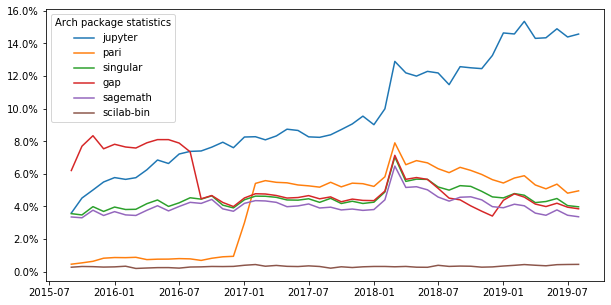
\includegraphics[width=0.9\textwidth]{arch-pkgstats.png}
    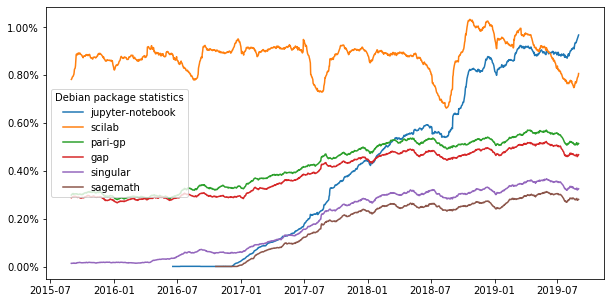
\includegraphics[width=0.9\textwidth]{debian-pkgstats.png}
    \caption{Arch and Debian package statistics for the project
      duration (2015-2019).}
    \label{fig:pkgstats}
  \end{figure}

  The ``popularity contests''\footnote{Public statistics on package
    use, based on voluntary submissions by users.} organized by the
  various Linux distributions give widely different numbers,
  reflecting the varying interests of the communities tied to each
  distribution. Figure~\ref{fig:pkgstats} shows historical package
  installation statistics for the duration of \ODK in Arch and Debian
  (the only distributions that make historical data
  available). Non-historical data for Ubuntu shows a similar trend to
  Debian. These figures are based on voluntary reporting, and are thus
  subject to important biases; nevertheless, we observe an increase in
  adoption of \ODK packages starting in 2017, in particular for
  \Jupyter.
  
  Because Jupyter is used in many research areas outside of
  mathematics, it is interesting to compare the percentage of ODK
  users to that of Jupyter users. For example, in 2019, in the Arch
  Linux distribution 34\% of Jupyter users are also \ODK users; this
  percentage jumps to 58\% on Debian and Ubuntu. Both figures are down
  from their values in 2018, because, unsurprisingly, the popularity
  of \Jupyter is growing faster than that of other \ODK components.
  
  \noindent
  It is also (mildly) interesting to compare the number of
  \emph{pulls} on DockerHub for Jupyter and for \ODK's containers
  (available for GAP and SageMath). In 2018, Jupyter's
  \texttt{scipy-notebook} container has more than 1 million pulls,
  whereas ODK components have between 10 and 100 thousands.

  \noindent
  This numbers should be taken with a grain of salt, since they are
  automatically incremented by continuous integration/testing systems
  deployed by the projects themselves.

  \noindent
  \ODK has made most of its components available on Conda Forge. The
  SageMath 8.9 package currently has 25K downloads (compare to 750K
  downloads for Jupyter).
\end{enumerate}

\subsection{KPIs for Aim 3}

\begin{aim}
  Identify and promote best practices in computational mathematical research including: making results easily reproducible; producing
  reusable and easily accessible software; sharing data in a semantically sound way; exploiting and supporting the growing
  ecosystem of computational tools.
\end{aim}

\subsubsection{Success stories}

\begin{enumerate}
%\item Best practice and tools for correct and reproducible research
\item \textbf{Mike Croucher's talk ``Is your research software correct''}\\
  This excellent talk highlights crucial best practice whenever
  software is used in research, including open code and data sharing,
  automation, use of high level languages, software training, version
  control, pair programming, literate computing, or testing. A lot of
  the work in ODK relates to disseminating this set of best practice
  (\longWPref{dissem}), and enabling it through appropriate technology
  (\longWPref{UI}). Just to cite a few examples,
  \longdelivref{UI}{jupyter-collab}, and
  \longdelivref{UI}{jupyter-test} enable respectively version control
  and testing in the \Jupyter literate computing technology, while
  Mike's talk is and will be delivered in several of ODK's many
  training events.

\item \textbf{RSE Conference Workshop: ``Reproducible research with Jupyter''}
  (\href{https://opendreamkit.org/2018/03/07/opendreamkit-at-the-rse-conference/}{blog post})\\
  OpenDreamKit member, Tania Allard, ran a hands-on workshop on
  Jupyter notebooks for reproducible research at the UK RSE
  Conference. This workshop focused on the use of Jupyter notebooks as
  a means to disseminate reproducible analysis workflows and how this
  can be leveraged using tools such as nbdime and nbval. Both nbdime
  and nbval were developed by members of the OpenDreamKit project as a
  response to the growing popularity of the Jupyter notebooks and the
  lack of native integration between these technologies and existing
  version control and validation/testing tools. An exceptional win was
  that this workshop was, in fact, \textbf{one of the most popular events of
  the conference} and we were asked to run it twice as it was massively
  oversubscribed. This reflects, on one hand, the popularity of
  Jupyter notebooks due to the boom of literate programming and its
  focus on human-readable code. Allowing researchers to share their
  findings and the code they used along the way in a compelling
  narrative. On the other hand, it demonstrates the importance of
  reproducible science and the need for tools that help RSE and
  researchers to achieve this goal, which aligns perfectly with the
  goals of OpenDreamKit.
  %

\item \textbf{Best presentation: 3D at the rescue for visualizing large mathematical ontologies}
  \href{https://opendreamkit.org/2018/08/20/tgview3d.md}{blog post}\\
  The Math-in-the-Middle (MitM) ontology and the system API theories
  in the MitM paradigm are big theory graphs with thousands of nodes
  and edges. Understanding and interacting with such large and complex
  objects is very difficult.The FAU group has conducted research into
  whether virtual reality technologies are helpful for this task. We
  have presented a first working prototype at the Conference on
  Intelligent Computer Mathematics CICM 2018 and the author: Richard
  Marcus - a master's student at FAU has received a prize for best
  presentation.
\item \textbf{Explainer cartoon on publishing reproducible logbooks}
  \href{https://opendreamkit.org/2017/11/02/use-case-publishing-reproducible-notebooks/}{cartoon}\\
  As part of our training and dissemination activities, we authored a
  series of Use Case blog posts: examples of applications that have
  been made possible through the OpenDreamKit project. The most
  important ones are illustrated by an explainer cartoon authored by
  Juliette Belin, graphic designer originally working at Logilab and
  nowadays as free-lance. The
  \href{https://opendreamkit.org/2017/11/02/use-case-publishing-reproducible-notebooks/}{cartoon}
  about Binder was retweeted by Chris Holdgraf from the Binder team:
  \emph{``I love this visual description of BinderHub from @JulietteTaka -
  obviously I'm a fan of Binder itself, but it's particularly great to
  see a visual take on the subject! I'd love for the open community to
  find more ways to invite these kinds of non-code contributions!''}.
  It had much success and we henceforth received several requests for
  reuse:
  \begin{itemize}
  \item Becky Arnold, from the Alan Turing Institute, London, UK, for
    \href{https://the-turing-way.netlify.com/reproducible_environments/04/binder/}{The
      Turing Way}, \emph{a lightly opinionated guide to reproducible
      data science}.
  \item Mark Hanly PhD, Lecturer at Centre for Big Data Research in
    Health of the University of Sydney, for ``a report I am preparing
    for the \href{https://ardc.edu.au/}{Australian Research Data
      Commons} and aims to inform how the ARDC can support researchers
    to use platforms like Jupyter Notebooks and Binder to disseminate
    their research. Juliette's cartoon is a very effective way to
    communicate the motivation and workflow; congratulations on an
    excellent visualisation!''.
  \item Sarah Gibson, from the Alan Turing Institute, London, UK, for
    a blog post
    ``\href{https://blog.jupyter.org/diving-into-leadership-to-build-push-button-code-df2a075c9914}{Diving
      into Leadership to Build Push-Button Code for BinderHub}''.
  \item Enol Fernandez, Gergely Sipos, from the EGI fundation for a
    \href{https://www.slideshare.net/EGI_Foundation/reproducible-open-science-with-egi-notebooks-binder-and-zenodo}{EOSC-Hub talk ``Reproducible Open Science with EGI Notebooks, Binder and Zenodo''}.
  \end{itemize}
\end{enumerate}

%Some research paper that showcases a range of best practices supported by ODK work (paper written collaboratively on e.g. github, software distributed as e.g. SageMath package, live demo and logbooks on binder, nbdime for collaboration, ...).

% \subsubsection{Use Case blog posts}

% As part of our training and dissemination activities, we have authored
% a series of Use Case blog posts: examples of applications that have
% been made possible through the OpenDreamKit project. For each one, we
% provide a brief tutorial on how to tackle it OpenDreamKit supported
% tools, link to some examples, and suggest best practices. The most
% important ones are illustrated by an explainer cartoon authored by
% Juliette Belin, graphic designer originally working at Logilab and
% nowadays as free-lance.

% \begin{enumerate}
% %4 use cases: %see:https://opendreamkit.org/tag/use-case
% \item \textbf{Publishing reproducible logbooks}
%   \href{https://opendreamkit.org/2017/11/02/use-case-publishing-reproducible-notebooks}{blog post}
% \item \textbf{Live online slides with SageMath, Jupyter notebooks, RISE and Binder}
%   \href{https://opendreamkit.org/2018/07/23/live-online-slides-with-sagemath-jupyter-rise-binder/}{blog post}
% \item \textbf{WP6 Math-in-the-Middle Integration Use Case}
%   \href{https://opendreamkit.org/2017/10/15/WP6-Usecase/}{blog post}\\
%   Two papers published at MACIS-2017
% \item \textbf{Mixing Data and Computation to explore mathematical data sets: Knowledge to the rescue with LMFDB + SageMath + Pari + MitM}
%   \href{https://opendreamkit.org/2018/05/16/lmfdb-usecase/}{blog post}
% % \item https://opendreamkit.org/2018/03/15/jupyterhub-binder-convergence/
% \end{enumerate}


\subsubsection{Quantitative metrics}

\begin{enumerate}
\item \textbf{GAP packages: activity and adoption of best practices}\\
  GAP has a powerful extension system that allows users to share their
  research code through an official channel. Thanks to GAP's
  continuous integration/testing, extension developers have been
  encouraged and helped to keep their code up to date. The \emph{code
    coverage}\footnote{Percentage of code covered by tests} of GAP has
  gone up from 69\% for the 4.9 release, to 75\% for the 4.10 release.
  During the year 2018, 50\% of GAP extension packages had been
  updated; by June 2019 this number had grown to 80\%.
\item \textbf{SageMath packages on PyPI}\\
  Following the lead of GAP, SageMath has been advocating, with the
  support of OpenDreamKit, the Python package repository PyPI for
  users to share their research code. This channel is still in its
  infancy. In 2015 there were a handful of packages on PyPI for
  SageMath; in 2018 the number grew to 117.
  \ednote{make a table, and add 2019}

\item \textbf{Systems made interoperable with the Math-in-the-Middle architecture}\\
  % More generally: metrics on the scale of the Math-in-the-Middle
  % architecture; e.g. number of API CDs generated and number of
  % alignements the current state of play is that we have initial
  % exports of system interface ontologies for three systems:
  The Math-in-the-Middle interoperability architectures is a
  foundational new way of making open-API systems interoperable
  (see~\cite{ODK-D6.5} for an overview). Thanks to a fully functional
  prototype integrating GAP, SAGE, SINGULAR, and LMFDB via the SCSCP
  Protocol, users can run calculations involving any combination of
  those systems from any of them.

  The following numbers highlight the state of play as of M36 (details in~\cite{ODK-D6.8}):
  \begin{compactdesc}
  \item[MitM-connected Systems] four (GAP, Sage, LMFDB, Singular)(See D6.5);
    % Upcoming: OEIS, FindStat
  \item[Formal MitM Ontology] 55 files, 2600 LoF, 360 commits (See D6.8);
  \item[Informal MitM Ontology] 815 theories, 1700 concepts in
    English, German,(Romanian, Chinese);
  \item[MitM System API Theories (GAP, Sage, LMFDB, Singular)] 1.000+;
    Theories, 22.000 Concepts;
  \item[SageMath Ontology] 512 CDs with 2800 entries;
  \item[GAP Ontology] 218 CDs with 2996 entries.
  \item[data.mathhub.info] six new datasets with together about 11M mathemtical objects
    with between 6 and 16 computed properties. Provenance sketches for all of them, one
    formalized in MMT.
  \end{compactdesc}

%In the course of the deliberations in the WP6 workshops we saw a shift from the development of computational foundations and verification towards API/Interface function specifications to enable semantic system interoperability via the Math-in-the-Middle Ontology. Consequently, emphasis has changed to the generation of API Content Dictionaries (API CDs) for GAP, LMFDB and SAGE. We have a prototypical set of GAP and SAGE Content Dictionaries in OMDoc/MMT form (GAP: 218 CDs, 2996 entries; SAGE: 512 CDs, 2800 entries overall). The computational foundations exist but are rather more simple than originally anticipated. Much of the functionality has been offloaded to the SCSCP standard – remote procedure call with OpenMath representations of the mathematical objects – developed in the SCIENCE Project. As a direct consequence of the work in OpenDreamKit the OpenMath Society has promoted the SCSCP protocol into as an OpenMath Standard.Conversely, the GAP and SAGE CDs are rather more elaborated than anticipated in the proposal, and thus form a viable basis for alignment with the MitM Ontology.
% https://github.com/OpenDreamKit/OpenDreamKit/blob/88ee2544e31e661c4eac7f39fa7333f24b62ab2a/terminations/report/wp6.tex
%https://github.com/OpenDreamKit/OpenDreamKit.github.io/blob/333b21524f753dd49e441b4b1157ded68999eeff/meetings/2018-02-01-SteeringCommitteeMeeting/ProgressReports/Zurich.md
\end{enumerate}

\subsection{KPIs for Aim 4}

\begin{aim}
  Maximise sustainability and impact in mathematics, neighbouring
  fields, and scientific computing.
\end{aim}

\subsubsection{OpenDreamKit's web site statistics}

\begin{itemize}
  % 7 activities on the website
\item 6 video interviews totaling 600 views % 400 in 2018
\item 6 press releases
\item 35 blogs (32 blogs and 3 technical blogposts)
\item 517 Twitter followers, 1862 tweets
\item Official website visitor statistics have been collected since
  March 2017, the visitor breakdown by year and country is reported in
  Table~\ref{tab:byregion}.
\end{itemize}

\begin{table}[h]
  \centering
  \begin{tabular}{l r r r r r}
    & {\bf 2016--2017} & {\bf 2017--2018} & {\bf 2018--2019} & \multicolumn{2}{c}{\bf Total}\\
    \hline
    North America   & 1,504 & 3,638 & 8,069 & 13,211 & 53.2\%\\
    Europe          &   936 & 2,745 & 5,354 &  9,035 & 36.4\%\\
    Asia            &    98 &   353 & 1,244 &  1,682 &  6.8\%\\
    Unknown         &    85 &   145 &   297 &    540 &  2.2\%\\
    South America   &    11 &    43 &   211 &    265 &  1.1\%\\
    Oceania         &     4 &    29 &    53 &     86 &  0.3\%\\
    Africa          &       &    12 &    18 &     30 &  0.1\%\\
    Central America &       &     3 &     1 &      4 &  0\%\\
    \hline
    {\bf Total}  & 2,638 & 2,795 & 6,968 & 15,247 & 24,853
  \end{tabular}
  \caption{Visits to \url{https://opendreamkit.org/}, by region and by year.}
  \label{tab:byregion}
\end{table}

\subsubsection{Workshops, conferences, events}

% Statistics on workshops organized and conference presentations
% delivered as part of our dissemination activities, including
% estimates of number of attendees and what (if anything) happened as
% a follow-up.

An important part of the success of the ODK project is linked to its
ability to foster a community in the spirit of the open source
projects it is built on. Part of this relies on the organization and
participation to scientific and development events of many different
scales and objectives.

Over the last four years OpenDreamKit has organized or coorganized 110
events:
\begin{itemize}
\item 5 project meetings
\item 24 development workshops
\item 45 training and building community workshops or sessions 
( including 5 targeted at women and 10 in developing countries) adding 1800 trainees
\item 7 research workshops
\end{itemize}
In addition, we communicated at and participated to 30 external events.

\subsubsection{Diversity success stories}
\label{diversity_success_stories}

\begin{enumerate}
\item \textbf{Women in \Sage workshops} \href{https://opendreamkit.org/2017/04/06/WomenInSage/}{blog post}\\
  The under-representation of women in the scientific world is even
  more visible if we intersect science with software development. During the four years of the projects we have organzided 5 events primarily targeted at women as to help form a team of women developers and to reduce the gap between men and women developers in Sage Math in particular and in open scientific software in general. Over 290 women received training.

  On January 2017, Viviane Pons, Jessica Striker and Jennifer
  Balakrishnan organized the first WomenInSage event in Europe with
  OpenDreamKit. 20 women spent a week together coding and learning in
  a rented house in the Paris area. We took advantage of the diverse
  knowledge background of our group to work together and learn from
  each other. It was an occasion for many "first times" among
  participants who had very little experience with Sage.

  This sparked the organization of another Women in Sage workshop in
  Montreal in June 2018. OpenDreamKit organized a new one in April 2019
  in Crete. It was co-organized by Eleni Tzanaki who had been a participant in the 
  2017 Women in Sage event. It was also an occasion to organize \Sage sessions
  at University of Crete and to add \Sage to the math curriculum.

\item \textbf{Women in computing}\\
  In partnership with CodeFirstGirls, OpenDreamKit developed training
  materials and provided training for over 130 women during Year 3 at Sheffield and Manchester

\item \textbf{ODK RSE Tania Allard was invited by NumFocus to
    participate in the Diversity and Inclusion in Scientific Computing
    unconference}

\item \textbf{ODK RSE Tania Allard diversity chair for the 2017
    International Research Software Engineering conference.}

\item \textbf{Training workshops in developing countries }\\
  10 training workshops were organized in developing countries
  including Algeria, Lebanon, Tunisia, Morocco, Colombia, Mexico, Nigeria and
  attended by about 460 trainees.\\
  
  The story of our event in Nigeria is particularly telling of the 
  dissemination work we do. Indeed, we first met Ini Adinya from University of Ibadan at the
  CIRM conference \emph{Free Computational Mathematics} organized by \ODK in February 2019. She 
  was there along with two other Nigerian mathematicians who had received funding from \ODK to attend. 
  They were thrilled by the conference and we decided to organize a \Sage workshop at Ibadan the 
  following summer where we welcomed 80 participants mostly from Nigeria and neighboring countries.
  
  The Workshop was run by Erik Madisson Bray from \ODK along with Yaé Ulrich Gaba, Evans Doe Ocansey, and Dr. Chimere 
  Stanley Anabanti. The three extra instructors had been found through \Sage mailing lists and community. They had prior
  experience with teaching \Sage in Africa but, to our knowledge, it was the first time that such an event was held in Nigeria.
  The workshop itself was a technical challenge with unreliable network and power outages but the impact on the attendees was
  undeniable. Actually, the most frequent feedback we got on our questionnaire was that the workshop should have lasted more than 
  a week! You can read more about the workshop on our blogpost here: \url{https://opendreamkit.org/2019/07/29/SageDays102/}.
\end{enumerate}

\subsubsection{Adoption of ODK technologies for teaching}

As reported on in \longdelivref{dissem}{IntroODK}, \OpenDreamKit
participants taught, or trained colleagues to teach, more than 30
courses each year at their home institutions using \OpenDreamKit
technology. Over the course of the project, \textbf{this impacted more
  than five thousand students}.

We report below on some success stories.

\begin{enumerate}
\item \textbf{African Institute for Mathematical sciences}\\
  In early spring 2017, Prof.~Dr.~W.~Decker and Prof.~Dr.~G.~Pfister
  gave a three-week course on computational algebraic geometry at the
  African Institute for Mathematical sciences (Cape Town, South
  Africa) with lectures and computer lab sessions. The course was
  attended by about 50 students from all over Africa. In the lab
  sessions, the students learned how to experiment with the computer
  algebra system Singular. It proved extremely valuable that the
  students could run Singular in the Jupyter notebook.

\item \textbf{PGTC "Software tools for mathematics" workshop 2018}\\
  Alexander Konovolov used GAP Jupyter interface in teaching
  Reproducible GAP experiments on Binder.
  % Here https://github.com/alex-konovalov
  % /gap-teaching, you can find a collection of GAP Jupyter notebooks. It uses the Docker container with the latest public release of GAP, which
  % is maintained in a separate repository at https://github.com/gap-system/gap-docker.

\item \textbf{University of Granada}\\
  The \GAP Jupyter kernel was used by Pedro Garcia-Sanchez to teach a
  master course in mathematical software at the University of Granada.
  See
  \url{https://github.com/pedritomelenas/Software-Matematicas-GAP}.
  Pedro has taken on the technology, and is now involved in the
  development of interactive visualization widgets for discrete maths
  (package Francy; see
  also~\longdelivref{UI}{ipython-advanced-interacts}) in particular
  for use in other courses.

\item \textbf{ Bioinformatics Awareness Days}\\
An event that took place in The Sheffield Institute for Translational Neuroscience on November 2017 where were given training activities
about bioinformatics workflows using Jupyter notebooks with
computation provided by the free Micosost Azure Notebook service. The event
demonstrated that \ODK supported technologies could be applied to the field of Bioinformatics and led to a new collaboration between Dr
Cutillo and \ODK member Mike Croucher.

Following the success of this workshop, Dr Cutillo independently taught an introductory workshop on statistics using Jupyter notebooks
on Azure at Parthenope University of Naples (Materials at \url{https://github.com/luisacutillo78/RbasicStats}) Dr Cutillo has since moved
to University of Leeds where she will be teaching statistics to 200+ undergraduates. She plans to use \ODK developed technologies
in collaboration with the Research Software Engineering group at Leeds.

The event required also the development of a website that was linked to the Jupyter notebooks (\url{https://bitsandchips.me/BAD_days/}). The
website caught the attention of Eleni Vasilaki, Head of Machine Learning at University of Sheffield who wanted to do something similar for
her course on Adaptive Intelligence. We supported her in this endeavour and the result is at (\url{http://bitsandchips.me
/COM3240_Adaptive_Intelligence/}).

In order to better support this, \ODK member Tania Allard, developed a Jekyll template for use by academics and researchers using Jupyter
notebooks for course materials and dissemination. This led to the development of a Python package: nbjekyll (\url{https://github.com
/trallard/nbjekyll}) that complements the Jekyll template. As well as being used internally at Sheffield, The nbjekyll package received some
attention on twitter \url{https://twitter.com/jdblischak/status/1009800776305332224} and \url{https://twitter.com/walkingrandomly/status
/1009414151716909057} receiving a total of 42 retweets and 80 'likes'% ( à remettre à jour).
\end{enumerate}

\subsubsection{Impact of some tools developed by OpenDreamKit}

% TODO: Stories about the impact of the Micromagnetics VRE;
% TODO: D4.13 (Sphinx) might have impact beyond ODK. For example, Simon King
%       is interested in things done for D4.13 for his
%       \software{p\_group\_cohomology} package. It might also lead to a PEP,
%       which by itself counts as impact.

%Vidar Fauske PRESENTATION filling in for Benjamin Ragan-Kelley during Second OpenDreamKit Review, on October 30, 2018 in Luxembourg
%https://opendreamkit.org/meetings/2018-10-28-Luxembourg/ProjectReview/wp4.pdf
%TODO: Could you please add more narrative text or more context? the information below appears in your presentation but listed that way this is too technical.

Measuring success of software can be a challenge.
One way to measure is to observe metrics of engagement on
a public development platform such as GitHub.
A 'star' means that an individual is following development of the project.
Issues are used to discuss the project, e.g. to report bugs, ask questions, request features, etc..
Comments indicate how much people are discussing the project,
and the number of authors of commits and discussion comments indicates
how broadly we are reaching.
Note that the number of participants in development discussion tends to be a very small fraction of total users,
which is difficult to estimate.
To compare, the Jupyter project estimates millions of users,
while the flagship notebook repository sees only thousands of participants on the repository in the last twelve months.

We report success for some \ODK components related to WorkPackage 4,
showing significant community engagement,
comparing the results to the previous twelve months,
showing an increase in popularity over time.

\begin{enumerate}
\item \textbf{nbdime}: Tool for diffing Jupyter notebooks\\
  GitHub statistics: 1336 stars on GitHub, 61 contributors (45 in 12
  months prior), 388 comments, 107 new issues (94 closed). Delivered
  in the first period (D4.6), \software{nbdime} has been met with
  enthusiasm and widely adopted. This led to further developments,
  including integration in the Jupyter Notebook,
  Jupyter Lab, and the version control git through extensions.
\item \textbf{Thebelab}: Jupyter-based javascript library for integrating live code in static web pages\\
  GitHub statistics: 96 stars, 28 contributors (15 in 12 months prior), 124 new issues (126 closed), 292 comments.\\
  Thebelab has been integrated into documentation tools such as jupyter-sphinx plugin
  and the documentation of several software packages,
  including some \SageMath documentation and other software beyond the \ODK consortium.
\item \textbf{K3D-Jupyter}: 3D visualisation in the Jupyter notebook.\\
  GitHub statistics: 131 stars, 14 contributors, 140 new issues (129 closed), 303 comments. \\
  This visualization tool is now used by \ODK component ubermag
  for interactive visualisation in Jupyter notebooks.
\end{enumerate}

%%% Local Variables:
%%% mode: latex
%%% TeX-master: "report"
%%% End:

%  LocalWords:  subsubsection textbf noindent Jupyter's Jupyter Enol Simulagora Logilab
%  LocalWords:  Simulagor visualization IPython visualization compactitem Logipedia
